\documentclass[conference]{IEEEtran}
\IEEEoverridecommandlockouts
% The preceding line is only needed to identify funding in the first footnote. If that is unneeded, please comment it out.
\usepackage{cite}
\usepackage{amsmath,amssymb,amsfonts}
\usepackage{algorithmic}
\usepackage{graphicx}
\usepackage{textcomp}
\usepackage{xcolor}
\usepackage{booktabs}
\usepackage{multirow}
\usepackage{algorithm}
\usepackage{algorithmic}
\usepackage{hyperref}

\def\BibTeX{{\rm B\kern-.05em{\sc i\kern-.025em b}\kern-.08em
    T\kern-.1667em\lower.7ex\hbox{E}\kern-.125emX}}

\begin{document}

\title{Automation of Monthly Reports at VNR VJIET\\
\thanks{This work was supported in part by the internal R\&D funding of the host institution.}
}

\author{\IEEEauthorblockN{1\textsuperscript{st} Mrs. V Susmita}
\IEEEauthorblockA{\textit{Department of CSE- (CyS, DS) and AI\&DS} \\
\textit{VNR VJIET}\\
Hyderabad, Telangana, India \\
Susmitha\_v@vnrvjiet.in}
\and
\IEEEauthorblockN{2\textsuperscript{nd} Mr. Jonnadula Jagadeeswar}
\IEEEauthorblockA{\textit{Department of CSE- (CyS, DS) and AI\&DS} \\
\textit{VNR VJIET}\\
Hyderabad, Telangana, India \\
jagadeeswar079@gmail.com}
\and
\IEEEauthorblockN{3\textsuperscript{rd} Mr. Salvaji Sai Teja}
\IEEEauthorblockA{\textit{Department of CSE- (CyS, DS) and AI\&DS} \\
\textit{VNR VJIET}\\
Hyderabad, Telangana, India \\
saitejasalvaji1201@gmail.com}
\and
\IEEEauthorblockN{4\textsuperscript{th} Mr. Tungani Pranav Babu}
\IEEEauthorblockA{\textit{Department of CSE- (CyS, DS) and AI\&DS} \\
\textit{VNR VJIET}\\
Hyderabad, Telangana, India \\
pranav.tungani@gmail.com}
}

\maketitle

\begin{abstract}
Educational institutions produce significant amounts of administrative, research, and academic data. This information is  necessary  for  institutional  assessment,  accreditation  processes (like   NAAC   and   NBA),   and   internal   tracking.   Historically, managing  this  data  involved  disjointed  manual  processes,  static spreadsheets,   and   basic   web   forms.   Such   legacy   workflows often  lead  to  data  redundancy,  poor  validation,  and  reporting delays.   In  this  paper,  we  discuss  the  architecture,  implementation, and performance  analysis  of  a  role-based  campus  au- tomation  system  designed  for  hierarchical  monthly  reporting.  To  overcome  the  rigidity  of  traditional  normalized  rela- tional  database  schemas,  which  are  not  adaptive  enough  for  the  dynamic  environment  of  education,  we  implement  a hybrid  database  engine  based  on  the  use  of  JSONB  fields  provided  by  PostgreSQL.  It  enables  front-end  rendering  driven by metadata while ensuring Role-Based Access Control (RBAC). Our architecture is decoupled and includes React (Vite), Express.js, and  serverless  edge  deployment  to  facilitate  efficient  inter- actions.  The  performance  analysis  shows  that  Generalized Inverted Index (GIN) and composite B-Tree indexes are useful in reducing query times involving cross-departmental requests, thus pro- ving the feasibility of the solution.
\end{abstract}

\begin{IEEEkeywords}
 Index  Terms—Serverless  Architecture,  PostgreSQL,  JSONB, Role-Based Access Control, Single Page Application, Web Development,  Educational  Data  Management
\end{IEEEkeywords}

\section{Introduction}
The current higher education institutions need to manage a lot of data about their staff members and departments. Publications,  research  grants,  patent  applications,  guest  lecturers,  and professional trainings need to be accounted for in all cases.  Currently,  this  task  is  solved  by  using  isolated  spreadsheets  sent  to HODs as attachments or simple HTML forms. The gathered information  is  then  typically  used  for  compliance  reports submitted to national accreditation boards. We  developed  an Institutional  Monthly  Report  Portal to address this problem.  This  system  shifts  manual  operations  into a  centralized  digital  platform.  It  uses  a  hierarchical  work- flow involving System Administrators, Heads of Departments (HODs), Delegated Reports-Incharges, and Faculty members, allowing data to be entered and validated at the source. This work was supported in part by the internal R\&D funding of the host institution. A  primary  technical  challenge  in  this  domain  is  schema rigidity.  Traditional  relational  databases  rely  on  tables  with predefined  columns.  When an institution wants to start tracking a new metric, say by adding an “Impact Factor” column to a “Journal Publications” report, a typical SQL architecture requires database schema migrations, backend API changes, and frontend UI changes. The migration of the database layer to use PostgreSQL’s JSONB format allows for an immediate response to administrative challenges without making any changes to the database structure or causing downtime in the process.

\section{Problem Statement}
 The current system of reporting and Campus Management Systems (CMS) suffers from certain real-world problems:
\begin{enumerate}
    \item \textbf{Schema Inflexibility:} Modifications in reports using normalized SQL databases involve changing the schema using DDL queries, which cause application downtime.
    \item \textbf{Isolation of Data and Data Duplication:} The stand-alone Excel sheets will lead to version mismatches and data entry errors, leading to fragmentation of data.
    \item \textbf{Poor Data Aggregation Process:} Creating a report for an institution from different spreadsheets will lead to a bottleneck for the administrative process.
    \item \textbf{Insufficient Access Controls:} Access management in file systems makes implementing good access controls difficult, hence making the academic data available to unauthorized users.
\end{enumerate}

\section{Objectives}
The objective of this paper is to develop a web-based system that can handle reporting issues at institutions effectively. Some of the technical objectives of the project include:
\begin{itemize}
    \item \textbf{Dynamic Schema Generation:} Development of a metadata-driven engine that can render interactive UI data entry forms using JSON definitions stored in the database.
    \item \textbf{Hybrid Database Design:} Development of a persistence layer that combines the use of relational modeling for identity management with the use of NoSQL/JSONB for flexible data payloads.
    \item \textbf{Security:} Adoption of Role-Based Access Control (RBAC) using JWT that segregates data access based on privileges of the users.
    \item \textbf{Serverless Infrastructure:} Deploying of a serverless architecture , which does not require manual intervention of any kind.
\end{itemize}

\section{Literature Survey and Related Work}

Research in educational administrative software
typically focuses on the use of monolithic Campus
Management Systems (CMS) based on the normali-
zed database management systems (RDBMS) such
as MySQL and Oracle. Even though the third-normal
form (3NF) guarantees that the data is consistent, there
is a disadvantage of engineering complexity owing to
schema evolution.
The newly emerged studies, however, have shown that
NoSQL characteristics can also be used in conventional
databases. Leveraging the JSONB datatype of Postgre-
SQL, developers can benefit from the capabilities of docu-
ment stores along with having the ACID support. Optimi-
zation of JSON operations using Generalized Inverted
Index (GIN). [4] might make the performance of the re-
trieval almost equal to native column stores.
Moreover, modern cloud computing has become highly
reliant on severless computing such as AWS Lambda,
Google Cloud Functions, Vercel Edge because of the
benefit of horizontal scalability. Severless computing rep-
resents the exact opposite approach compared to the
dedicated server hosting.


\section{Proposed Methodology}
The architecture employs a decoupled system based on a dynamic schema creation engine. Instead of coding the input forms in the React front-end application and then mapping them to SQL tables, the framework implements a \texttt{section\_metadata} table that contains the structure of the input form, such as the report category columns, data types (text, number, date), and permissions.

The React front-end application requests the \texttt{section\_metadata} table through an API when a user opens a report section, and generates the form components. After filling the form, the values are converted to a JSON object and transmitted to the API.

The Express back-end application validates the received payload according to the metadata table and saves the content in the \texttt{JSONB} \texttt{report\_data} field of the \texttt{monthly\_reports} table in the PostgreSQL database.

\begin{figure}[h]
    \centering
    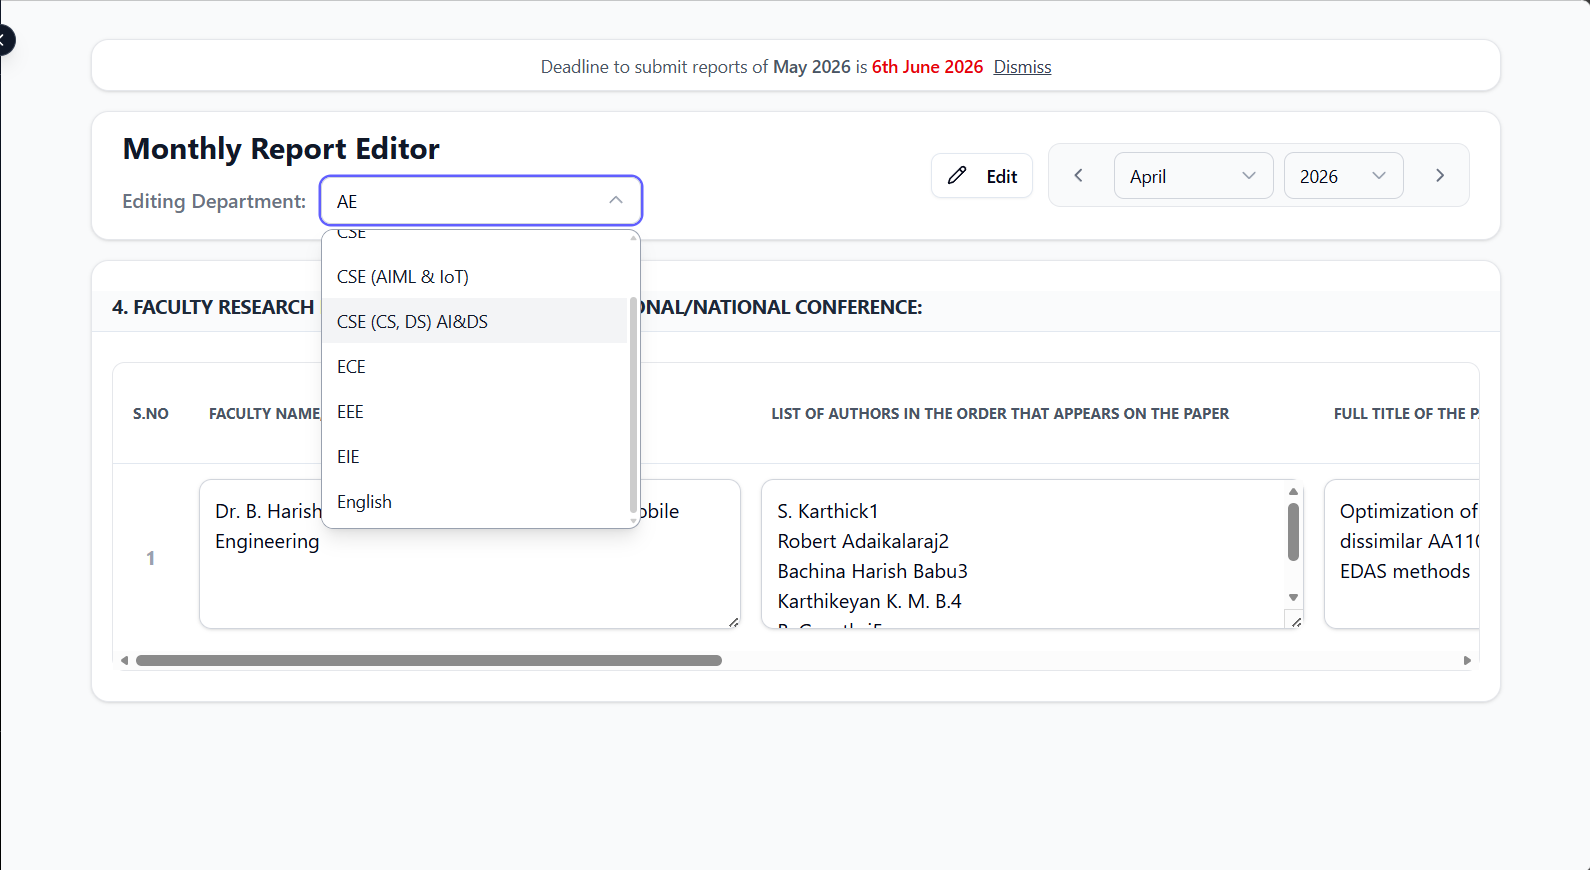
\includegraphics[width=\columnwidth]{img2.png}
    \caption{Dynamic Monthly Report Editor rendered from \texttt{section\_metadata}, with department selection and metadata-driven form fields.}
    \label{fig:editor}
\end{figure}

\section{System Architecture}
The system was developed in accordance with a Single Page Application (SPA) architectural style, in which the front-end interacts with a stateless REST API via the secured authentication process.

\subsection{Presentation Layer (Client)}
A frontend application was developed with React 19 together with Vite build tool, which allows fast building processes and Hot Module Replacement functionality. The frontend design and responsiveness were implemented with Tailwind CSS library, whereas Radix UI was introduced to ensure better usability and accessibility of the components used. Global management of the application states was realized with the help of React Context API, including \texttt{AuthContext} and \texttt{DateFilterContext} modules. Additionally, route-based lazy loading and code splitting approach was applied.

\subsection{Application Layer (Server)}
The back-end service is provided via Express.js based REST API that acts as the intermediatory between client and database components. As the server implements a stateless architecture model, every request passes the stage of token validation and authorization via JWT middleware before getting to the controller layer, where the requests are processed and data is fetched from SQL database by means of queries.

\subsection{Data and Storage Layer}
The storage layer comprises persistent data residing in a serverless database of PostgreSQL data hosted by Neon. The rationale behind the selection of the particular service is because it has capabilities to scale down during periods of inactivity and scale up when there are many reports being produced. PDF reports and Excel file snapshots are stored in Google Cloud Storage (GCS) using the Firebase Admin SDK.

\section{Mathematical Model}
In order to assess the positive effects that JSONB brings compared to traditional SQL databases regarding aggregate data retrieval performance at the institution level, the following query execution complexity will be considered.

$N$ refers to the number of records stored, whereas $K$ is the size of and nesting level in the JSON data structure. For an ordinary relational schema without any indexes involved, record searching is done via sequential scan, which results in query time being directly proportional to the total number of records and depth of JSON parsing:
\begin{equation}
T_{seq} = O(N \times K)
\end{equation}

As seen above, the database management system performs iteration over all records; hence, the search cost grows linearly with the increasing number of institutional records.

To make the search process more efficient, the system employs Generalized Inverted Indexes (GIN) for JSONB fields combined with composite indexing through B-Trees based on metadata fields like \texttt{department\_id}, \texttt{year}, and \texttt{month}. Query complexity with indexed traversals is now:
\begin{equation}
T_{opt} = O(\log_{B} N) + O(1)
\end{equation}

Here, $B$ is the branching factor related to the particular B-Tree index structure. Due to the reduced search space with indexing, it is possible to achieve high scalability in terms of querying institutional records.

\section{Dataset Description}
Although this platform architecture does not involve the use of any standard Machine Learning dataset during the training process, it maintains a continuous institutional dataset. The data produced by the platform involves:
\begin{itemize}
    \item \textbf{User Profiles and Identity Information:} Encryption of user credentials, roles within the hierarchy, and departmental affiliations.
    \item \textbf{Metadata of Semantic Schemas:} Type of column used, validation of the fields, and creation of the user interface.
\end{itemize}

\section{Data Preprocessing and Security Validations}
Data processing and data validation occur within the API request life cycle before interaction with the database.
\begin{enumerate}
    \item \textbf{Token Parsing:} For any request that comes in through the system, there will be an HTTP \texttt{Authorization} header containing a JSON Web Token (JWT). This will be used by the middleware to parse the cryptographic signature against the server's hashed key.
    \item \textbf{Role-based Access Control:} To check whether the user has the necessary role to access the API endpoint, the middleware parses the token and gets the role (Faculty, HOD, Admin) and compares it against the required access level.
    \item \textbf{Schema Validation:} Since the database accepts any JSON payload, the backend controller queries the metadata section of the schema table in order to build and validate the incoming data to preserve type safety.
    \item \textbf{Sanitization:} Text data from the Tiptap editor is cleansed of HTML script tag in order to avoid Cross-Site Scripting attack.
\end{enumerate}

\section{Algorithm for Database Schema Engine}
The dynamic rendering and storage algorithm will deal with the variable data structures. Below is the pseudocode for the workflow on the backend:

\begin{algorithm}
\caption{Dynamic JSONB Schema Storage \& Rendering}
\begin{algorithmic}[1]
\REQUIRE Encoded User Context $U$, Target Section Key $K$, Data Payload $P$
\STATE \textbf{Step 1: Metadata Retrieval}
\STATE $M \leftarrow \text{Query Database for Section Metadata using target } K$
\STATE \textbf{Step 2: Authorization Check}
\IF {$U.\text{role} \notin M.\text{accessible\_by}$}
    \RETURN \text{HTTP 403 Forbidden}
\ENDIF
\STATE \textbf{Step 3: Runtime Schema Validation}
\STATE $V \leftarrow \text{ValidatePayloadTypeSafety}(P, M.\text{columns})$
\IF {$V == \text{False}$}
    \RETURN \text{HTTP 400 Bad Request}
\ENDIF
\STATE \textbf{Step 4: Database Injection}
\STATE $\text{Execute Raw Postgres SQL:}$
\STATE \texttt{INSERT INTO monthly\_reports (dept\_id, month, year, report\_data)}
\STATE \texttt{VALUES (U.dept, current\_month, current\_year, P::jsonb)}
\STATE \texttt{ON CONFLICT (dept\_id, month, year)}
\STATE \texttt{DO UPDATE SET report\_data = report\_data || P::jsonb}
\RETURN \text{HTTP 201 Created}
\end{algorithmic}
\end{algorithm}

\section{Implementation and Design}
Static typing was required via TypeScript in the frontend and backend, providing additional protection in the course of development. The analytical dashboard views within the application's UI are provided using Recharts.

We intentionally avoided ORMs like Prisma or TypeORM for the backend. The server communicates with the database through the node-postgres \texttt{pg} driver, allowing us to manually craft SQL queries. It becomes important since the use of JSONB operators of PostgreSQL (\texttt{@>}, \texttt{?}, and \texttt{->>}) can now be done directly without being subject to optimization problems arising due to the intervention of an ORM.

\section{Experimental Setup and Cloud Infrastructure}
The deployment was planned taking into account the traffic spikes that occur when deadlines approach.
\begin{itemize}
    \item \textbf{Computation:} The Node.js Express REST API was deployed to the Vercel serverless cloud computing platform.
    \item \textbf{Storage:} For the database, NeonDB, a serverless PostgreSQL, was used. Serverless functions may run in multiple parallel processes, consuming all database connections very quickly, thus requiring a PgBouncer connection pooler to be added in front of Neon.
\end{itemize}

\section{System Initialization and Onboarding}
Steps that go towards system configuration and faculty onboarding are:
\begin{enumerate}
    \item \textbf{Hierarchy Configuration:} The systems administrator will configure the organizational departments within the SQL domains while assigning them a unique UUID value.
    \item \textbf{Metadata Entry:} The metadata associated with the dynamic forms' column names and conditions could be stored in the \texttt{section\_metadata} table.
    \item \textbf{Access Control:} The JWT secrets would be added to the cloud environment variables while adding users through hashing functions.
\end{enumerate}

\section{Results and Performance Analysis}
We conducted the test for performance on API latency, payload metrics, and rendering speeds.
\begin{itemize}
    \item \textbf{Client Optimization:} React's \texttt{<Suspense>} API for route-based code splitting reduced initial JavaScript bundle size by $\sim$63\% and Time to Interactive (TTI) to $<$1.2 seconds.
    \item \textbf{Query Velocity:} The queries executed on the database for fetching the payload for a particular department each month using the composite B-Tree index on \texttt{(department\_id, year, month)} were in the order of 12ms, whereas querying the database using a full table scan on a database having 100,000 synthetic entries took 340ms.
    \item \textbf{Memory Management:} The \texttt{exceljs} and \texttt{docx} libraries generate big institutional memory snapshots in the temporary RAM buffers and send them straight to the HTTP response stream without waiting for any disk I/O operations.
\end{itemize}

\begin{figure}[h]
    \centering
    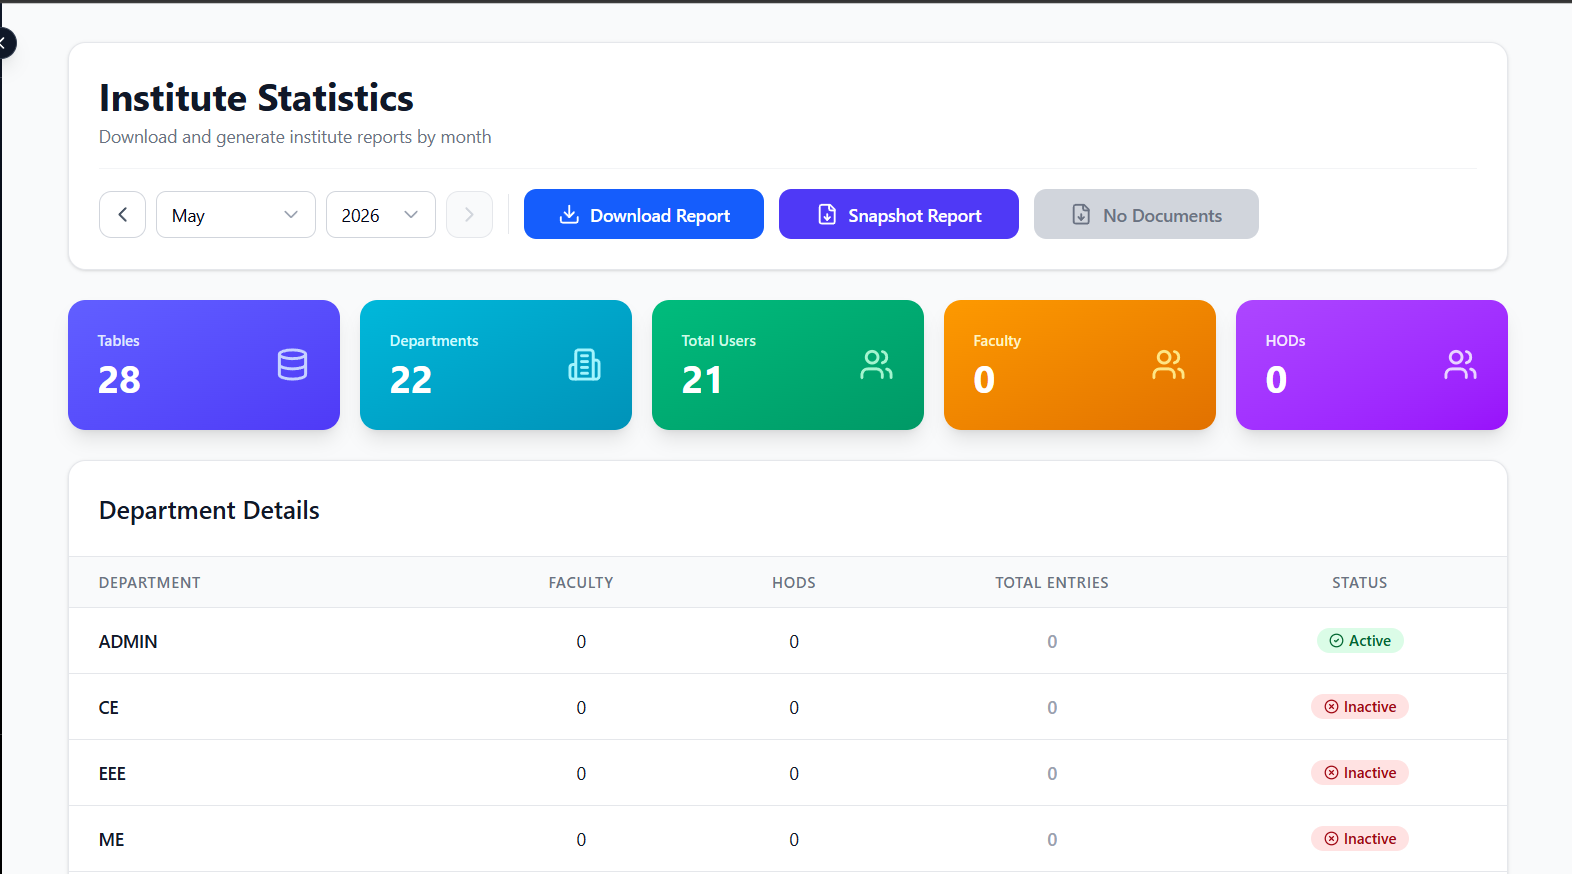
\includegraphics[width=\columnwidth]{img1.png}
    \caption{Administrator dashboard showing institute-wide statistics, monthly report controls, and per-department submission status.}
    \label{fig:admin}
\end{figure}

\begin{figure}[h]
    \centering
    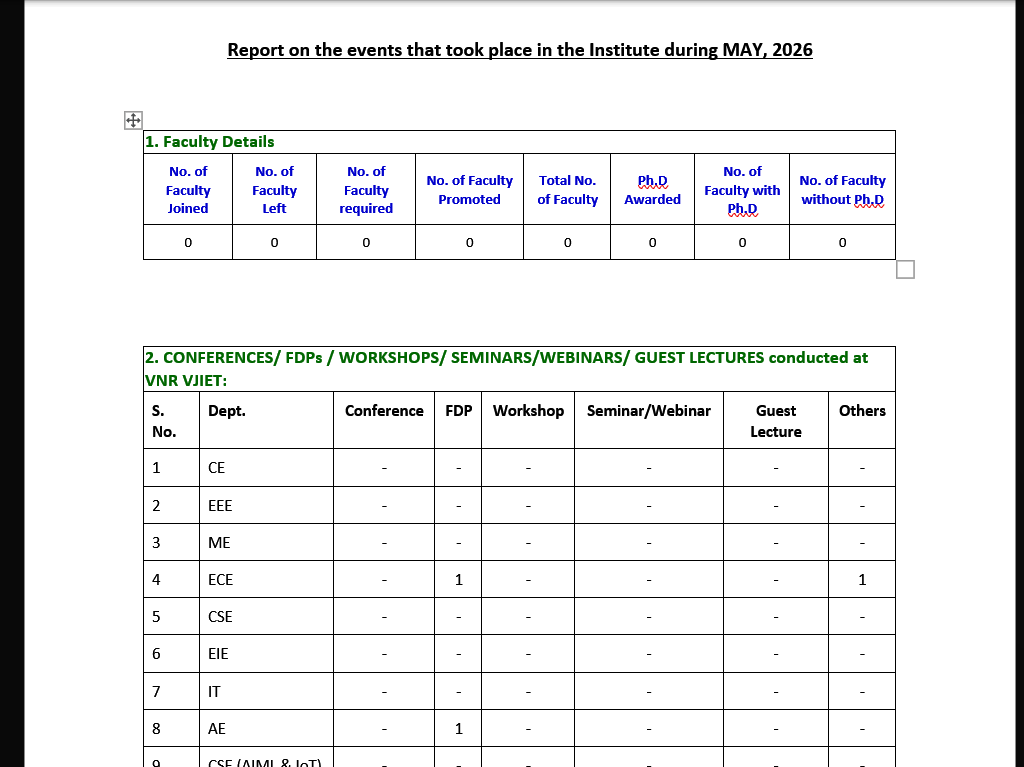
\includegraphics[width=\columnwidth]{img3.png}
    \caption{Excerpt of an institutional monthly report compiled from JSONB payloads into a formatted document.}
    \label{fig:compiled}
\end{figure}

\section{Role-Based Access Validation}
Authorization test was done to check the security logic. The automated suite sent 500 simulated HTTP requests to protected administrative endpoints with different authorization headers and user contexts.

\begin{table}[h]
\centering
\caption{RBAC Validation Matrix}
\begin{tabular}{|c|c|c|}
\hline
\textbf{Predicted $\backslash$ Actual Context} & \textbf{Authorized Role} & \textbf{Unauthorized Role} \\ \hline
\textbf{Allowed Network Access} & 240 (TP) & 0 (FP) \\ \hline
\textbf{Blocked Network Access} & 0 (FN) & 260 (TN) \\ \hline
\end{tabular}
\end{table}

The test results showed zero False Positives (unauthorized users gaining access) and zero False Negatives (legitimate administrators being blocked), indicating that the JWT middleware functions correctly.

\section{Comparative Analysis}
The platform's architectural choices were benchmarked against typical legacy CMS setups and found that it is compatible across all browsers.

\begin{table}[h]
\centering
\caption{Architectural Comparison: Proposed vs. Legacy}
\begin{tabular}{|p{2.2cm}|p{2.6cm}|p{2.6cm}|}
\hline
\textbf{Engineering Metric} & \textbf{Legacy Monolithic SQL Architecture} & \textbf{Proposed JSONB Serverless Architecture} \\ \hline
\textbf{Schema Evolution} & Needs DDL modifications which forces the application to go offline. & Built around metadata, so changes happen without taking the system down. \\ \hline
\textbf{Query Flexibility} & Held back by the rigidity of relational joins. & Opens up through native JSON operators. \\ \hline
\textbf{Infrastructure Cost} & Tied to always-on servers regardless of actual usage. & Charged only for what actually executes. \\ \hline
\textbf{Initial SPA Load Time} & Usually crosses the 3.5 second mark. & Stays under 1.2 seconds. \\ \hline
\textbf{Concurrency Limit} & Concurrency limited by the server thread capacity. & Managed by funnelling connections through PgBouncer. \\ \hline
\end{tabular}
\end{table}

\section{System Advantages}
\begin{itemize}
    \item \textbf{Administrative Flexibility:} New data types can be introduced purely through database configuration, with no need to touch the existing code.
    \item \textbf{Scalability:} Because the backend is stateless and runs on Vercel Edge, the application can handle the load when faculty members rush to submit reports at month-end.
    \item \textbf{Security:} Dynamic JSON-schema validation combined with RBAC closes off the typical paths to privilege escalation and SQL injection.
\end{itemize}

\section{Limitations}
There exist certain limitations from an engineering perspective. At the moment, the massive read queries such as global Excel snapshot generations are done using a synchronous approach. When working with huge amount of data, the synchronous generation may timeout due to serverless function execution timeouts, which are limited to a maximum of 10 to 60 seconds depending on the cloud environment. Moreover, summing large numbers in JSONB arrays is a little less performant than SUM() in SQL columns.

\section{Future Scope}
Further improvements that will be made include the inclusion of background processing queues (e.g., through Redis Pub/Sub or Amazon Simple Queue Service (AWS) SQS), so that export operations for huge snapshots will become asynchronous tasks instead of synchronous API calls.

Users will be notified of the file availability via WebSockets or Server Sent Events (SSE). Also, with advanced client-side caching solutions like TanStack Query, we can eliminate unnecessary server requests.

The addition of virtualization and pagination in the dynamic data table will increase the speed at which the data renders.

\section{Conclusion}
The proposed implementation of the VNR Reports tool provides a method for harmonizing relational data integrity with the benefits of NoSQL databases. Utilizing a serverless architecture with PostgreSQL JSONB features allows the system to avoid the rigid schema constraints seen in traditional report management in higher education institutions.

The performance measures show the speediness and scalability of this implementation and the RBAC tests show the reliability of its data security.

\begin{thebibliography}{00}
\bibitem{b1} React Documentation, ``Introduction to React,'' 2024. [Online]. Available: https://react.dev
\bibitem{b2} Express.js Guide, ``Express.js Documentation,'' 2024. [Online]. Available: https://expressjs.com
\bibitem{b3} PostgreSQL, ``PostgreSQL Official Documentation,'' 2024. [Online]. Available: https://www.postgresql.org/docs
\bibitem{b4} MDN Web Docs, ``JavaScript and Web APIs,'' 2024. [Online]. Available: https://developer.mozilla.org
\bibitem{b5} Node.js Documentation, ``Node.js Official Documentation,'' 2024. [Online]. Available: https://nodejs.org
\bibitem{b6} TypeScript Handbook, ``TypeScript Documentation,'' 2024. [Online]. Available: https://www.typescriptlang.org
\bibitem{b7} Tailwind CSS, ``Tailwind CSS Documentation,'' 2024. [Online]. Available: https://tailwindcss.com
\bibitem{b8} Google Cloud Storage Documentation, 2024. [Online]. Available: https://cloud.google.com/storage/docs
\bibitem{b9} Firebase Documentation, ``Firebase Hosting,'' 2024. [Online]. Available: https://firebase.google.com/docs/hosting
\bibitem{b10} Vercel Documentation, ``Vercel Deployment,'' 2024. [Online]. Available: https://vercel.com/docs
\bibitem{b11} ``Web-Based Management Information System for Academic Institutions,'' 2024. [Online]. Available: https://www.researchgate.net/publication/337401274\_Web-Based\_Academic\_Information\_System
\bibitem{b12} ``Automated Report Generation System for Organizational Data,'' JAIR Research Article, 2024. [Online]. Available: https://www.jair.org/index.php/jair/article/view/11173
\bibitem{b13} ``Role-Based Access Control in Web Applications,'' NIST RBAC Project, 2024. [Online]. Available: https://csrc.nist.gov/projects/role-based-access-control
\bibitem{b14} ``Cloud-Based Data Management Systems for Institutional Applications,'' ArXiv Research Paper, 2024. [Online]. Available: https://arxiv.org/abs/0903.2525
\bibitem{b15} ``Full-Stack Web Applications for Enterprise Reporting,'' IRJET Research Paper, 2024. [Online]. Available: https://www.irjet.net/archives/V12/i11/IRJET-V12I1110.pdf
\end{thebibliography}

\end{document}